%%%%%%%%%%%%%%%%%%%%%%%%%%%%%%%%%%%%%%%%%%%%%%%%%%%%%%%%%%%%%%%%%%%%%%%%
% Preamble
%%%%%%%%%%%%%%%%%%%%%%%%%%%%%%%%%%%%%%%%%%%%%%%%%%%%%%%%%%%%%%%%%%%%%%%%
\documentclass[11pt]{article}
%
% Packages and other includes
% Pagination
\usepackage[letterpaper, margin=1in]{geometry}
\usepackage{emptypage}
\usepackage{mhchem,ulem}
%
% Fonts
\usepackage[T1]{fontenc} % best for Western European languages
\usepackage{lmodern} % Latin Modern instead of CM
\usepackage{textcomp} % required to get special symbols
%
% Math
\usepackage{amsmath, amssymb}
\usepackage{braket}
%
% Graphics, floats, tables
\usepackage{graphicx, xcolor, float, array}
%
% Hyperlinks
\usepackage{hyperref}
%
%
% Definitions and settings
% Paragraph indent and spacing
\setlength{\parskip}{0.4\baselineskip}
\setlength{\parindent}{0in}
\newcommand{\brian}[1]{
  {\begin{quote}
      \color{blue} #1
  \end{quote}}
}
%
%
% Title, authors, date
\title{\textbf{Midterm 2b Problems}}
%
%
%%%%%%%%%%%%%%%%%%%%%%%%%%%%%%%%%%%%%%%%%%%%%%%%%%%%%%%%%%%%%%%%%%%%%%%%
% Main document
%%%%%%%%%%%%%%%%%%%%%%%%%%%%%%%%%%%%%%%%%%%%%%%%%%%%%%%%%%%%%%%%%%%%%%%%
%

\begin{document}

\maketitle

1. \textbf{Equilibrium Constants} Determine $K_c$ at 25$^\circ$C
for the reaction,
\begin{center}
  \ce{N$_2$(g) + O$_2$(g) + Cl$_2$(g) <=> 2 NOCl(g)},
\end{center}
given the following data set at 25$^\circ$C. Report result to 2 significant figures.
\begin{center}
  \ce{N$_2$(g) + 2 O$_2$(g) <=> 2 NO$_2$(g) $\,\,$ $K_p = 1.0\times 10^{-18}$ atm$^{-1}$}

  \ce{2 NOCl(g) + O$_2$(g) <=> 2 NO$_2$Cl(g) $\,\,$ $K_p = 1.21\times 10^4$ atm$^{-1}$}

  \ce{2 NO$_2$(g) + Cl$_2$(g) <=> 2 NO$_2$Cl(g) $\,\,$ $K_p = 9.0\times 10^{-2}$ atm$^{-1}$}
\end{center}

\brian{Invert the second equation and take the product. The overall $K_p = 7.4\times 10^{-24}$ atm$^{-1}$
  and $K_c = 3.0 \times 10^{-25}$ M$^{-1}$
  }

2. \textbf{Essay Question: Gibbs Free Energy} Explain in a few sentences why the Gibbs
free energy is a central quantity in chemical thermodynamics. What type(s) of information
can be obtained from the Gibbs free energy change of a process? Name at least two methods
for determining the Gibbs free energy of a chemical reaction experimentally, computationally,
or using tabulated data.

\brian{Delta G also gives the amount of available work (at constant pressure).
  It also determines the equilibrium constant and provides the direction or ``driving force''
  for a reaction to achieve equilibrium. Two ways of determining the Gibbs free energy of a reaction:
  \begin{enumerate}
  \item $\Delta G = \Delta H^\circ_r - T\Delta S^\circ_r$ where $\Delta H^\circ_r$ and $\Delta S^\circ_r$
    are the standard enthalpy and standard entropy of reaction. These are determined from tabulated
    standard enthalpy and standard entropy of formation. $T$ is the temperature
  \item $\Delta G^\circ_r = \sum_i \nu_i\Delta G^\circ_f(P_i)-\sum_i\nu_i(R_i)\Delta G^\circ_f(R_i)$
    using tabulated standard free energies of formation $\Delta G^\circ_f$ and cofficients of the reaction
    $\nu$
  \end{enumerate}
}

3. \textbf{Entropy} Does the entropy of the system/reaction mixture increase,
decrease, or stay the same in the following processes? Briefly explain your
answer in each case.

a) Isothermal expansion of a fixed amount of an ideal gas

\brian{Entropy increases since the volume increases
  \begin{equation*}
    \Delta S = R\ln\frac{V_f}{V_i}
  \end{equation*}
  where $V_f$ and $V_i$ are the final and initial states, respectively.
}

b) Haber-Bosch synthesis of ammonia

\brian{N$_2$(g) + 3 H$_2$(g) $\rightleftharpoons$ 2 NH$_3$(g)

  Entropy decreases since there are fewer moles of products than reactants
}

c) Evaporation of a liquid

\brian{Entropy increases since gases occupy greater volume}

d) Mixing of fixed amounts of two chemically different ideal gases at constant temperature, 
total pressure, and total volume

\brian{Entropy increases since partial pressures of the gases decreases upon mixing.}

4. \textbf{Van't Hoff Equation} In the gas phase, nitrosyl chloride NOCl is in chemical
equilibrium with its dissociation products, nitrogen monoxide and chlorine gas.

\begin{table}[hbpt]
  \centering
  \begin{tabular}{lll}
      & $\Delta H^\circ_f$ (kJ/mol) & $\Delta S^\circ$ (J/(mol K)) \\
      \hline
      NO     & 90.29 & 210.76 \\
      ClNO   & 51.71 & 261.68 \\
      Cl$_2$ &       & 223.08
  \end{tabular}
  \caption{Thermochemical data at standard conditions.}
  \label{tab:therm}
\end{table}

a) Formulate the balanced chemical equation including states.

\brian{2 NOCl(g) $\rightleftharpoons$ 2 NO(g) + Cl$_2$(g)}

b) Using the thermochemical data from Table \ref{tab:therm}, estimate the temperature $T_c$
at which the equilibrium constant $K$ equals 1.

\brian{Use the following equation
  \begin{equation*}
      \ln K = -\frac{\Delta H^\circ}{RT} + \frac{\Delta S^\circ}{R}
  \end{equation*}
  and determine $\Delta H^\circ = 77.16$ kJ/mol and $\Delta S^\circ=121.96$ J/(mol K). The
  temperature at which $K=1$ is 633 K.
}

c) Qualitatively plot $\ln K$ as a function of $1/T$ based on your results from (b).

\begin{center}
  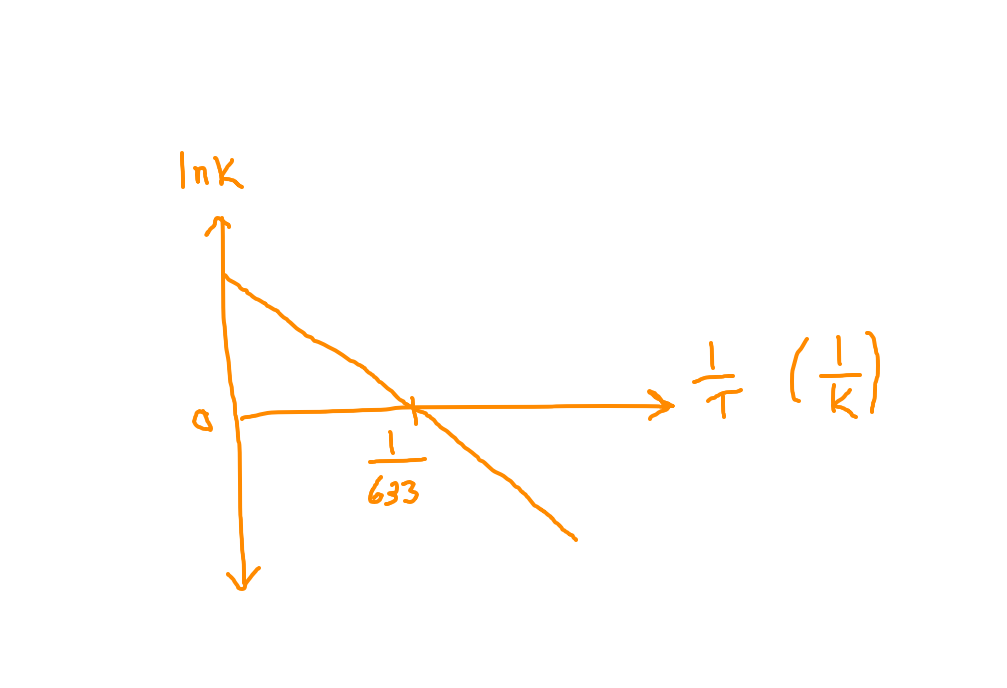
\includegraphics[scale=0.4]{vant_hoff.png}
\end{center}

%{\color{blu-1e} d) Using the plot in c), at what temperature range is the product favored for the
%  dissociation of NOCl? Briefly explain your answer.}
%
%\brian{Temperatures above 238 K will favor the dissociation of NOCl. Because $\Delta H^\circ > 0$,
%  the reaction is endothermic and this means that $K$ increases with increasing temperature.
%}

5. \textbf{Statistical Thermodynamics} 1.5 mol of ethyne (a.k.a. acetylene, C$_2$H$_2$) gas
are kept in a 1 L steel cylinder. Assume ideal behavor.

a) Determine the total entalpy of the sample at 300 K.

\brian{$U = H - PV$ at constant pressure $P$ and $H$ is the total enthalpy. Quadratic degree
  of freedom $f_q = 5 $. Hence, $U = \frac{5}{2}nRT$ and using ideal gas $PV = nRT$

  \begin{align*}
    H = & U + PV \\
    = & U + nRT \\
    = & \frac{5}{2}nRT + nRT \\
    = & (\frac{5}{2} + 1)(1.5\times 0.08206 \times 300) \\
    = &  \text{129.2445 L atm} = 13.1 \text{ kJ}
  \end{align*}  
}

b) The pressure of the sample is doubled by reducing the volume to 0.5 L. The
temperature is kept constant. Determine the total enthalpy.

\brian{13.1 kJ}

c) Estimate the root mean square (rms) velocity of the ethyne molecules in m/s at 300 K.
The mass of a single ethyne molecule is $4.324\times 10^{-26}$ kg.

\brian{
  \begin{align*}
    \frac{1}{2}mv^2_\text{rms} = & \frac{3}{2}kT \\
    v_\text{rms} = & \sqrt{\frac{3}{4.324\times 10^{-26}}(1.3806\times 10^{-23})(300)} \\
    v_\text{rms} = & 536 \text{ m/s}
  \end{align*}
}

d) Determine the entropy change when the original gas sample is heated from 300 K to
800 K.

\brian{Determing $C_v = f_q\frac{1}{2}nR$
  \begin{align*}
    \Delta S = & C_v\ln\frac{T_f}{T_i} \\
    = & 30.6 \text{ J/K}
  \end{align*}
}

e) Ethyne has a standard free energy of formation of 209.9 kJ/mol. Why is it not smart
to heat a pressurized steel cylinder containing ethyne?

\brian{The formation of C$_2$H$_2$ has chemical formula 2 C(s) + H$_2$(g)$\rightleftharpoons$ C$_2$H$_2$(g).
  It is spontaneous for the decomposition of C$_2$H$_2$(g) into the elements and releases free energy.
  H$_2$ is highly explosive.
}

\end{document}
